\section{Swarm Intelligence}

Swarm behavior is found in many different species in nature, including fish schools and flocks of birds. Many of the species that practice swarm behavior does this because of a biological need to stay together. An example of this is that predators usually attacks one individual, and not an entire flock. This swarm behavior is also found in social insects like ants, wasps, bees and termites. They collaborate on tasks including building nests, gather food and organizing production. These social insect colonies have shown us that simple organisms can perform complex tasks by interacting with each other. The colonies are highly distributed and self-organized, and they adapt well to changes in the environment. Swarm intelligence \citep{beni89} is a branch of artificial intelligence that is strongly influenced by the swarm behavior found i nature, and it tries to adapt these characteristics in intelligent computer systems.

\subsection{Ant Colony Optimization}
In nature ants have proven to be extremely capable of finding an optimal or close to optimal route from the nest to a food source \citep{deneubourg90}. Ants communicate by leaving a pheromone trail that other ants are capable of smelling and follow by a certain probability. Most ant species leave a pheromone trail when retuning to the nest from an important food source, and the ants who decides to follow the same path also leave behind a pheromone trail. The more pheromone units on the trail (i.e. the more ants who choose the given path), the greater the probability the other ants will chose it. Because pheromone disappear over time, shorter paths will be favored over longer paths simply because shorter paths (usually) takes shorter time, and thus will have more pheromone units. 

Ant Colony Optimization (ACO) is a class of graph representation based metaheuristic algorithms designed to optimize routing problems. The first description of an ACO algorithm, called Ant System (AS), was initially proposed by \citet{dorigo96}. The AS strategy developed by Dorigo tries to simulate the behavior of real ants, but he adds several artificial characteristics including visibility, memory and discrete time. \citet{nanda11} described a generic implementation of the algorithm, as follows, where \textit{A} is the set of ants, \textit{E} is the set of edges in the graph, and $B \in E$ is the set of edges that form the best solution: \\

\begin{algorithm}[H]
 initialize\;
 \While{stop criteria are not met}{
  \ForAll{ants a in A}{
   position a in StartNode
  }
  \Repeat{every ant has a solution}{
   \ForAll{ants a in A}{
    choose nextNode\\* 
    $pheromone_{(currentNode,nextNode)}+=update$
   }
  }
  \ForAll{edges e in B}{
   $pheromone_e += deposit$
  }
  \ForAll{edges e in E}{
   $pheromone_e -= evaporation$
  }
 }
 \caption{Generic Ant Colony Optimization Algorithm}
\end{algorithm}


The idea of ACO algorithms is to create a decentralized system with multiple agents. The agents influence each others decisions using pheromones. In the beginning, before any distinct pheromone trail is laid, the ants choices are random and thus they perform a broad search in the environment. This randomness will decrease over time as the pheromone trails becomes more distinct. The literature describes many different algorithms that can be classified as ACO algorithms \citep{salehi-nezhad07,tripathi09,jiang10, dias14}, and most of authors describes artificial ants with additional features to those found in nature, including vision and memory. The addition of features is typically done to increase the performance of the algorithm and reduce some of the randomness in the beginning.  

%TODO: SKRIVE OM ACO I RUTEOPTIMALISERING! 

\subsection{Bee Colony Optimization}
As described in \citet{lucic03}, bees are capable of performing a variety of complex tasks. One of these tasks are the collection and processing of nectar, which may be considered as extremely organized. The idea is that a bee that leaves the hive to gather nectar, flies to the hives so-called dance floor. The bees that have already found a good food source performs a ``dance'' at the dance floor to advertise that they have found a satisfying source of food. The bee that just came from the hive chooses one of the dancing bees and flies with it to its food source. As stated in \citet{lucic03} the mechanism of deciding which bee to follow is not well understood, but it is considered that ``the recruitment among bees is always a function of the quality of the food source''. After the bee has gathered and returned the food to the hive, the bee has three options\citep{lucic03}:

\begin{enumerate}
  \item It can abandon the food source and return to the dance floor, and again become an uncommitted follower
  \item It can continue to gather nectar from the food source without recruiting nestmates
  \item It can return to the dance floor and dance, and thus recruit nestmates before returning to the food source
\end{enumerate}

Bee Colony Optimization (BCO) is metaheuristic methods, that like ACO, aims to create a decentralized optimization system with multiple agents, based on graph representation. The idea is to apply the collective intelligence of the food gathering process to an optimization system. Like a typical ACO algorithm, a typical BCO algorithm is inspired by the way bees acts in nature, but some of the features of natural bees are added to and removed from the artificial bee. \citet{nikolic14} describes a BCO algorithm where the artificial bee only has two options after returning from a ``food source'': (1) abandon or (2) recruit. \citet{lucic03} gives the artificial bees attributes such as memory and perfect knowledge about the quantity of nectar collected by other bees. Modifications like these can make the algorithms more efficient, and thus more suitable of performing complex combinatorial problems, like the Traveling Salesman Problem. 


\subsection{Particle Swarm Optimization}
%[TODO]: Skrive om PSO
% http://ieeexplore.ieee.org/stamp/stamp.jsp?tp=&arnumber=785511
As reported in \citet{shi99} Particle Swarm Optimization (PSO) was first introduced by Eberhart and Kennedy in 1995. PSO is inspired by the social behavior of flocks (such as flocks of birds) and schools (such as fish schools), and the idea is to update the population of individuals according to the individual's own experience and its companions' experience. This is unlike other evolutionary computational algorithms, like Genetic Algorithms, that uses evolutionary operators to manipulate the individuals. The basic concept is that each individual flies (or swims) with a certain velocity, and that this velocity is dynamically adjusted based on the experience. Each individual is a volume-less particle (i.e. point) in the D-dimensional search space. The \textit{i}th particle position is represented as $X_i = (X_{i1},X_{i2}...X_{iD})$. Each particle knows its own best position so far (the position that gave the highest fitness value), represented as $P_i = (P_{i1},P_{i2}...P_{iD})$, and the best position\textit{g}, achieved among all the particles. These two positions are used to calculate the velocity, $V_i = (V_{i1},V_{i2}...V_{iD})$ ,  of the \textit{i}th particle \citep{shi99}: 
\newline
\newline
\centerline{$V_{id} = w * V_{id} + c_1 * rand() * (P_{id}-X_{id}) + c_2 * Rand() * P_{gd}-X_{id})$}
\newline
\newline
where \textit{w} is a decreasing parameter called inertia weight brought to the PSO for balancing local and global search, $c_1$ and $c_2$ are two positive constants, and \textit{rand()} and \textit{Rand()} are two random functions in the range [0,1]. The new position of the \textit{i}th particle is calculated as follows \citep{shi99}:
\newline
\newline
\centerline{$X_i = X_{id} + V_{id}$}
\newline
\newline
Because of the decreasing inertia weight PSO may suffer from low global search ability at the end of the run, and may therefor be stuck at a local optima. Because of this PSO may fail to find the required optima when the problem to be solved is very complicated and complex \citep{shi99}. However, PSO has proven to solve NP hard problems including the Multi-Dimensional Knapsack Problem\citep{wan09}.

\begin{figure}[h!]
  \centering
  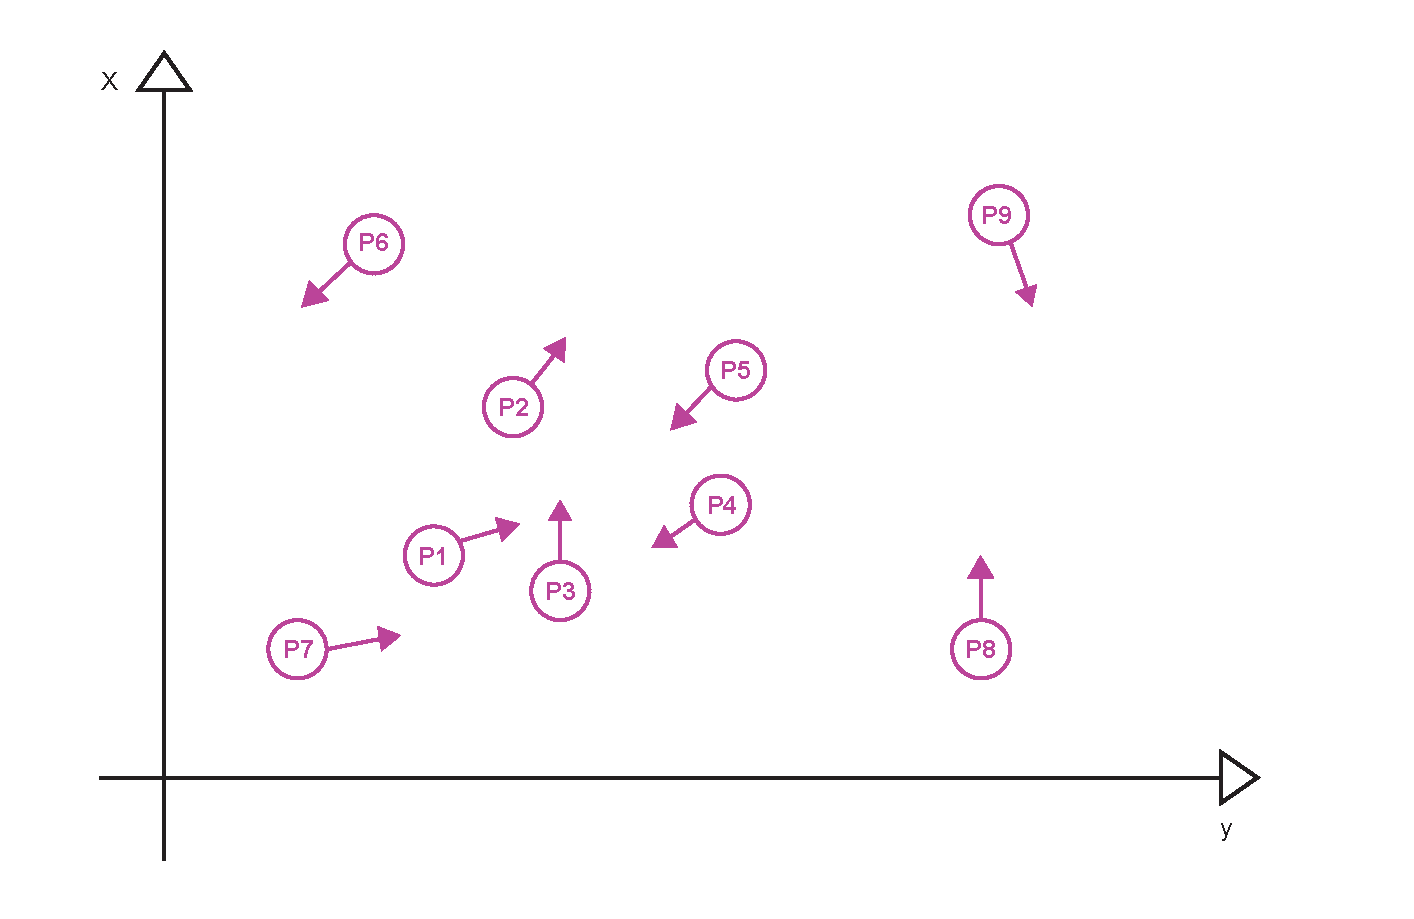
\includegraphics[width=4in]{assets/pso_diagram1.pdf}
  \caption[PSO1]
   {PSO diagram1} 
   \textit{}
\end{figure}

\begin{figure}[h!]
  \centering
  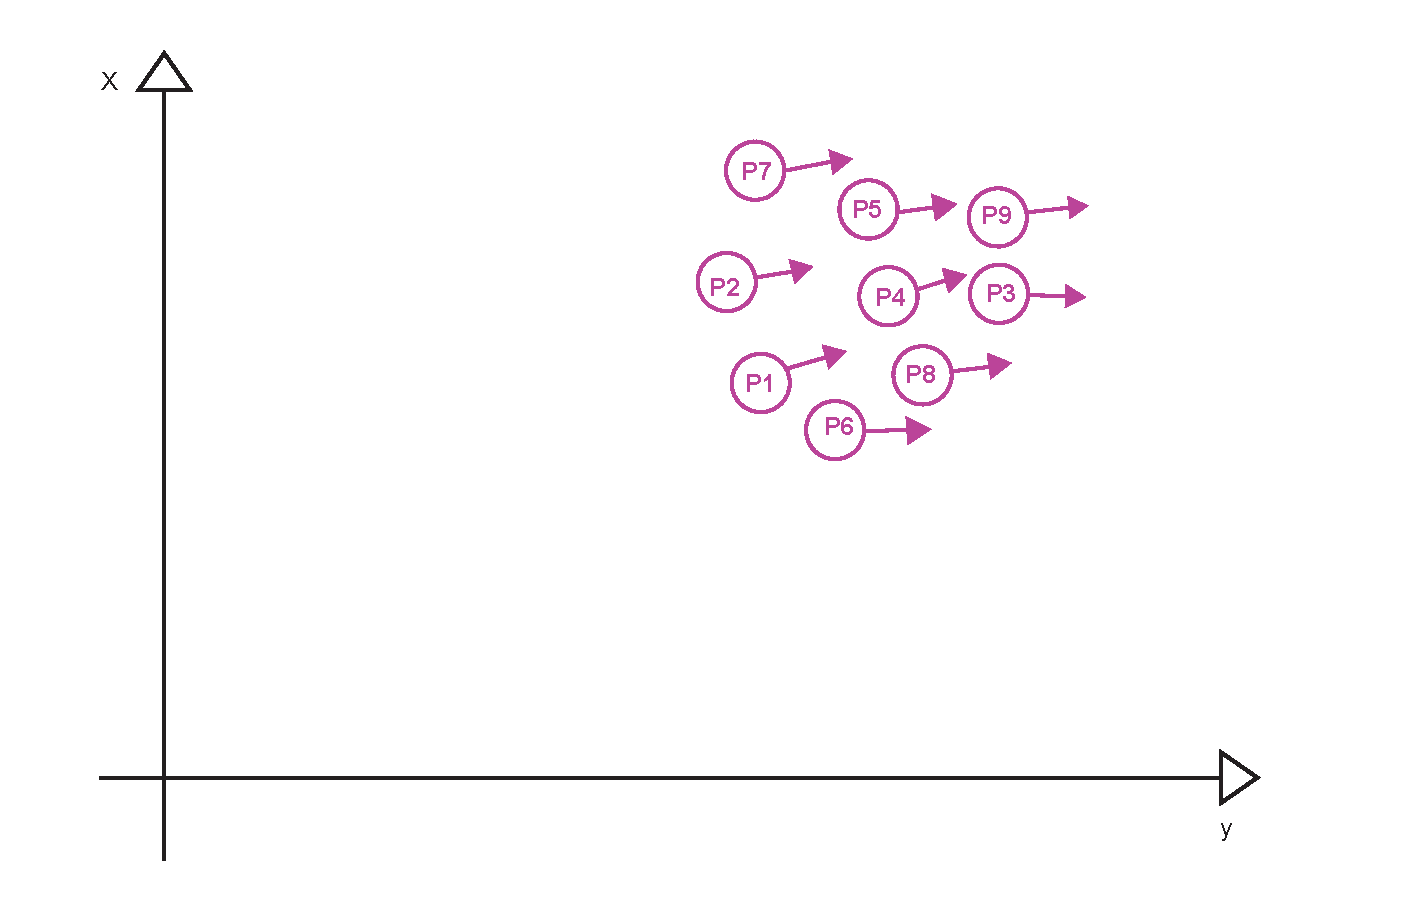
\includegraphics[width=4in]{assets/pso_diagram2.pdf}
  \caption[PSO2]
   {PSO diagram2} 
   \textit{}
\end{figure}




